\chapter{Isometries}

\begin{quote}
And since you know you cannot see yourself, so well as by reflection,
I, your glass, will modestly discover to yourself, that of yourself
which you yet know not of.

\hfill---William Shakespeare
\end{quote}




\section{Matrices as Functions}

We're going to discuss some basic functions in geometry.
Specifically, we will talk about translations, reflections, and
rotations. To start us off, we need a little background on
matrices.\index{matrix}

\begin{ques} 
What is a \textit{matrix}?
\end{ques}

You might think of a matrix as just a jumble of large brackets and
numbers. However, we are going to think of matrices as
\textit{functions}. Just as we write $f(x)$ for a function $f$ acting
on a number $x$, we'll write:
\[
\mat{M} \vec{p} = \vec{q} 
\]
to represent a matrix $\mat{M}$ mapping point $\vec{p}$ to point
$\vec{q}$. A point $\vec p$ is often represented as an ordered pair of
coordinates, $\vec{p} = (x,y)$. However, to make things work out
nicely, we need to write our points all straight and narrow, with a
little buddy at the end:
\[
(x,y) \leadsto \begin{bmatrix} 
x \\ 
y \\
1
\end{bmatrix}
\]
Throughout this chapter, we will abuse notation slightly, freely
interchanging several notations for a point:
\[
\vec{p} \leftrightsquigarrow
(x,y) \leftrightsquigarrow
\begin{bmatrix} 
x \\ 
y \\
1
\end{bmatrix}
\]
With this in mind, our work will be done via matrices and
points that look like this:
\[
\mat{M} = 
\begin{bmatrix}
a & b & c \\ 
d & e & f \\
0 & 0 & 1
\end{bmatrix}\qquad\text{and}\qquad \vec{p} = 
\begin{bmatrix}
x \\
y \\
1
\end{bmatrix}
\]
Now recall the nitty gritty details of \textit{matrix
  multiplication}:\index{matrix!multiplication}
\begin{align*}
\mat{M} \vec{p} &= 
\begin{bmatrix}
a & b & c \\ 
d & e & f \\
0 & 0 & 1
\end{bmatrix}
\begin{bmatrix}
x \\
y \\
1
\end{bmatrix} \\
&= \begin{bmatrix}
ax + by + c\cdot 1\\
dx + ey + f\cdot 1\\
0\cdot x + 0 \cdot y  + 1\cdot 1
\end{bmatrix}\\
&= \begin{bmatrix}
ax + by + c\\ 
dx + ey + f\\
1
\end{bmatrix}
\end{align*}

\begin{ques} Fine, but what does this have to do with geometry?
\end{ques}

In this chapter we are going to study a special type of functions,
called \textit{isometries}. These are function that preserves
distances. Let's see what we mean by this:

\begin{dfn} 
An \textbf{isometry}\index{isometry} is
a function $\mat{M}$ that maps points in the plane to other points in
the plane such that
\[
d(\vec{p}, \vec{q}) = d(\mat{M} \vec{p},\mat{M}\vec{q}),
\]
where $d$ is the distance function.
\end{dfn}


\begin{ques}
How do you compute the distance between two points again?
\end{ques}
\QM

We're going to see that several ideas in geometry, specifically
translations, reflections, and rotations which all seem very
different, are actually all isometries. Hence, we will
be thinking of these concepts as matrices.



\subsection{Translations}

Of all the isometries, \textit{translations} are probably the
easiest. With a translation, all we do is move our object in a
straight line, that is, every point in the plane is moved the same
distance and the same direction. Let's see what happens to Louie
Llama\index{Louie Llama} when he is translated:
\[
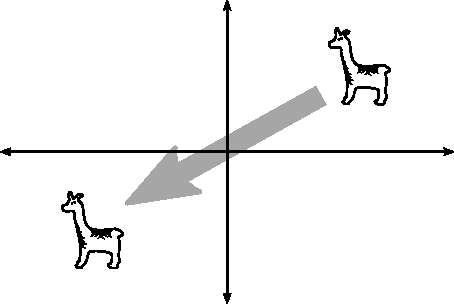
\includegraphics{../graphics/transIdeaEg.pdf}
\]

Pretty simple eh? We can give a more ``mathematical'' definition of a
translation involving our newly-found knowledge of matrices! Check it:

\begin{dfn}\index{translation}
A \textbf{translation}, denoted by $\mat{T}_{(u,v)}$, is a function
that moves every point a given distance $u$ in the $x$-direction and a
given distance $v$ in the $y$-direction. We will use the following
matrix to represent translations:
\[
\mat{T}_{(u,v)} = 
\begin{bmatrix}
1 & 0 & u \\ 
0 & 1 & v \\
0 & 0 & 1
\end{bmatrix}
\]
\end{dfn}


\begin{eg} 
Consider the point $\vec{p} = (-3,2)$. Use a matrix to translate
$\vec{p}$ $5$ units right and $4$ units down.
\[
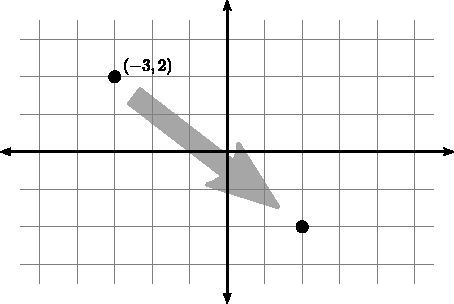
\includegraphics{../graphics/transEg1.pdf}
\]
Here is how you do it:
\begin{align*}
\mat{T}_{(5,-4)} \vec{p} &= 
\begin{bmatrix}
1 & 0 & 5 \\ 
0 & 1 & -4 \\
0 & 0 & 1
\end{bmatrix}
\begin{bmatrix}
-3 \\
2 \\
1
\end{bmatrix}\\
&=
\begin{bmatrix}
-3 + 0 + 5\\
0 + 2 - 4 \\
0 + 0 + 1
\end{bmatrix}\\
&=
\begin{bmatrix}
2\\
-2 \\
1
\end{bmatrix}
\end{align*}
Hence, we end up with the point $(2,-2)$. But you knew that already,
didn't you?
\end{eg}

\begin{ques} 
Can you demonstrate with algebra why translations are isometries?
\end{ques}
\QM


\begin{ques} 
We know how to translate individual points. How do we move entire
figures and other funky shapes?
\end{ques}
\QM


\subsection{Reflections}


The act of reflection has fascinated humanity for millennia.  It has a
strong effect on our perception of beauty and has a defined place in
art---not to mention how useful it is for the application
of make-up. Here is our definition of a reflection:

\begin{dfn}\index{reflection}
The \textbf{reflection} across a line $\l$, denoted by $\mat{F}_\l$, is the
function that maps a point $\vec{p}$ to a point $\mat{F}_\l
\vec{p}$ such that:
\begin{enumerate}
\item If $\vec{p}$ is on $\l$, then $\mat{F}_\l \vec{p} = \vec{p}$.
\item If $\vec{p}$ is not on $\l$, then $\l$ is the perpendicular
  bisector of the segment connecting $\vec{p}$ and $\mat{F}_\l \vec{p}$. 
\end{enumerate}
\end{dfn}

You might be saying, ``Huh?''  It's not as hard as it looks.  Check
out this picture of the situation, again Louie Llama\index{Louie Llama} 
will help us out:
\[
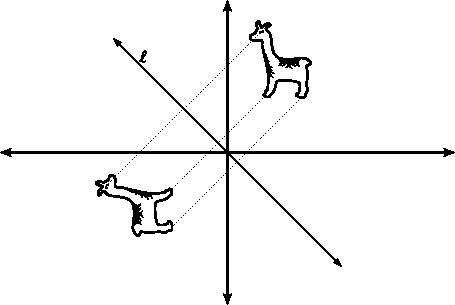
\includegraphics{../graphics/refIdeaEg.pdf}
\]

\subsubsection{A Collection of Reflections}

We are going to begin with a trio of reflections. We'll start with a
\textbf{horizontal reflection}\index{horizontal reflection}\index{reflection!horizontal} across the $y$-axis.  Using
our matrix notation, we write:
\[
\mat{F}_{x=0} =
\begin{bmatrix}
-1 & 0 & 0\\
 0 & 1 & 0\\
 0 & 0 & 1
\end{bmatrix}
\]

The next reflection in our collection is a \textbf{vertical
  reflection}\index{vertical reflection}\index{reflection!vertical}
across the $x$-axis.  Using our matrix notation, we write:
\[
\mat{F}_{y=0} =
\begin{bmatrix}
1 &  0 & 0\\
0 & -1 & 0\\
0 &  0 & 1
\end{bmatrix}
\]
The final reflection to add to our collection is a \textbf{diagonal
  reflection}\index{diagonal reflection}\index{reflection!diagonal}
across the line $y=x$.  Using our matrix notation, we write:
\[
\mat{F}_{y=x} =
\begin{bmatrix}
0 & 1 & 0\\
1 & 0 & 0\\
0 & 0 & 1
\end{bmatrix}
\]


\begin{eg}
Consider the point $\vec{p} =(3,-1)$.  Use a matrix to reflect
$\vec{p}$ across the line $y = x$.
\[
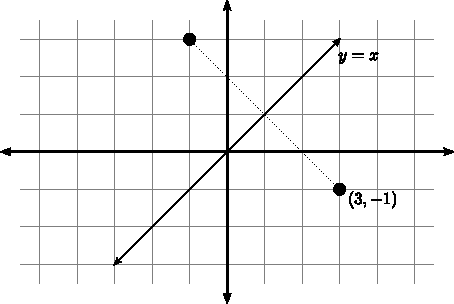
\includegraphics{../graphics/refEg1.pdf}
\]
Here is how you do it:
\begin{align*}
\mat{F}_{y = x} \vec{p} &= 
\begin{bmatrix}
0 & 1 & 0 \\ 
1 & 0 & 0 \\
0 & 0 & 1
\end{bmatrix}
\begin{bmatrix}
3 \\
-1 \\
1
\end{bmatrix}\\
&=
\begin{bmatrix}
0-1+0\\
3+0+0 \\
0+0+1
\end{bmatrix}\\
&=
\begin{bmatrix}
-1\\
3 \\
1
\end{bmatrix}
\end{align*}
Hence we end up with the point $(-1,3)$. 
\end{eg}

\begin{ques}
Let $\vec{p}$ be some point in Quadrant I of the $(x,y)$-plane. What
reflection will map this point to Quadrant II? What about Quadrant IV?
What about Quadrant III?
\end{ques}
\QM


\begin{ques} 
Can you demonstrate with algebra why each of our reflections above are
isometries?
\end{ques}
\QM




\subsection{Rotations}

Imagine that you are on a swing set, going higher and higher until you
are actually able to make a full circle\footnote{Face it, I think we
  all dreamed of doing that when we were little---or in my case, last
  week.}. At the point where you are directly above where you would be
if the swing were at rest, where is your head, comparatively?  Your
feet?  Your hands?


Rotations should bring circles to mind. This is not a
coincidence. Check out our definition of a \textit{rotation}:

\begin{dfn}\index{rotation}
A \textbf{rotation} of $\theta$ degrees about the origin, denoted by
$\mat{R}_\theta$, is a function that maps a point $\vec{p}$ to a point
$\mat{R}_\theta \vec{p}$ such that:
\begin{enumerate}
\item The points $\vec{p}$ and $\mat{R}_\theta \vec{p}$ are equidistant
  from the origin.
\item An angle of $\theta$ degrees is formed by $\vec{p}$, the origin, and
  $\mat{R}_\theta\vec{p}$.
\end{enumerate}
Louie Llama, can you do the honors?\index{Louie Llama}
\end{dfn}
\[
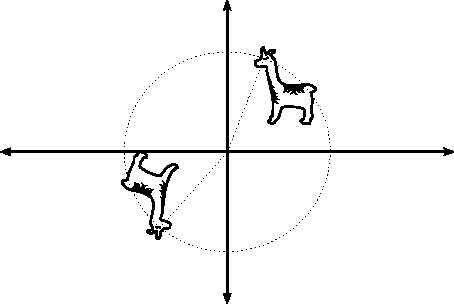
\includegraphics{../graphics/rotIdeaEg.pdf}
\]
\begin{war} 
Positive angles denote a counterclockwise rotation. Negative angles
denote a clockwise rotation.
\end{war}

Looking back on trigonometry, there were some angles that kept on
coming up. Some of these were $90^\circ$, $60^\circ$, and $45^\circ$.
We'll focus on these angles too.
\[
\mat{R}_{90} =
\begin{bmatrix}
0 & -1 & 0\\
1 & 0 & 0\\
0 & 0 & 1
\end{bmatrix}
\qquad 
\mat{R}_{60} =
\begin{bmatrix}
\frac{1}{2} & \frac{-\sqrt{3}}{2} & 0\\
\frac{\sqrt{3}}{2} & \frac{1}{2} & 0\\
0 & 0 & 1
\end{bmatrix}
\qquad
\mat{R}_{45} =
\begin{bmatrix}
\frac{1}{\sqrt{2}} & \frac{-1}{\sqrt{2}} & 0\\
\frac{1}{\sqrt{2}} & \frac{1}{\sqrt{2}} & 0\\
0 & 0 & 1
\end{bmatrix}
\]


\begin{eg} 
Consider the point $\vec{p} = (4,-2)$. Use a matrix to rotate
$\vec{p}$ $60^\circ$ about the origin.
\[
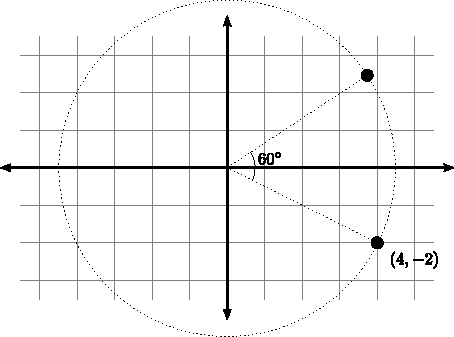
\includegraphics{../graphics/rotEg1.pdf}
\]
Here is how you do it:
\begin{align*}
\mat{R}_{60} \vec{p} &= 
\begin{bmatrix}
\frac{1}{2} & \frac{-\sqrt{3}}{2} & 0\\
\frac{\sqrt{3}}{2} & \frac{1}{2} & 0\\
0 & 0 & 1
\end{bmatrix}
\begin{bmatrix}
4 \\
-2 \\
1
\end{bmatrix}\\
&=
\begin{bmatrix}
2 +\sqrt{3} + 0\\
2\sqrt{3} -1 + 0 \\
0 + 0 + 1
\end{bmatrix}\\
&=
\begin{bmatrix}
2+\sqrt{3}\\
2\sqrt{3}-1 \\
1
\end{bmatrix}
\end{align*}
Hence, we end up with the point $(2+\sqrt{3},2\sqrt{3}-1)$.
\end{eg}


\begin{ques}
Do the numbers in the matrices above look familiar? If so, why?
\end{ques}
\QM

\begin{ques}
How do you rotate a point $180$ degrees?
\end{ques}
\QM


\begin{ques} 
Can you demonstrate with algebra why our rotations
above are isometries?
\end{ques}
\QM




\newpage


\problems
\begin{enumerate}
\item How do you compute the distance between two points $\vec{p}$ and
  $\vec{q}$ in the plane?
\item Use algebra to explain why: 
\[
d(\vec{p},\vec q) = d(\vec{p}-\vec q,\vec o) = d(\vec o,\vec{p}-\vec q)
\]
where $\vec o = (0,0)$.
\item What is an isometry?
\item What is a translation?
\item What is a rotation?
\item What is a reflection?
\item Reflecting back on this chapter, suppose I translate a point
  $\vec{p}$ to $\vec{p}'$. Does it make any difference if I move the
  point $\vec{p}$ along a wiggly path
\[
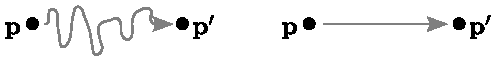
\includegraphics{../graphics/wiggle.pdf}
\]
or a straight path? Explain your reasoning.
\item Reflecting back on this chapter, is a rotation the continuous
  \textit{act} of \textit{moving} a point through an angle around some
  fixed point, or is it just a final picture compared to the initial
  one? Explain your reasoning.
\item In the vector illustrator \textit{Inkscape} there is an option
  to transform an image via a ``matrix.'' If you select this tool, you
  are presented with $6$ boxes to fill in with numbers:
\[
\begin{array}{|c|c|c|}
\hline
 & & \\
\hline
 & & \\
\hline
\end{array}
\]
Use what you've learned in this chapter to make a guess as to how this
tool works.
\item In what direction does a positive rotation occur?
\item Is a $270^\circ$ rotation the same as a $-90^\circ$ rotation?
  Explain your reasoning.
%\item Devise a way to explain translations using compass and
%  straightedge constructions.
%\item Devise a way to explain translations using origami
%  constructions.
%\item Devise a way to explain reflections using origami constructions.
%\item Devise a way to explain rotations using compass and straightedge
%  constructions.
\item Consider the following matrix:
\[
\mat{M} = 
\begin{bmatrix}
1 & 0 & 0\\
0 & 1 & 0\\
0 & 0 & 1
\end{bmatrix}
\]
Is $\mat{M}$ an isometry? Explain your reasoning.
\item Consider the following matrix:
\[
\mat{M} = 
\begin{bmatrix}
0 & 0 & 8\\
2 & 1 & 0\\
0 & 0 & 1
\end{bmatrix}
\]
Is $\mat{M}$ an isometry? Explain your reasoning.
\item Consider the following matrix:
\[
\mat{M} = 
\begin{bmatrix}
0  & -1  & 0\\
-1 & 0  & 0\\
0  & 0  & 1
\end{bmatrix}
\]
Is $\mat{M}$ an isometry? Explain your reasoning.
\item Consider the following matrix:
\[
\mat{M} = 
\begin{bmatrix}
0  & 2  & 0\\
-3 & 0  & 0\\
0  & 0  & 1
\end{bmatrix}
\]
\item Consider the following matrix:
\[
\mat{M} = 
\begin{bmatrix}
1  & 2  & 1\\
1 & 1  & 2\\
0  & 0  & 1
\end{bmatrix}
\]
Is $\mat{M}$ an isometry? Explain your reasoning.
\item Use a matrix to translate the point $(-1,6)$ three units right
  and two units up. Sketch this situation and explain your reasoning.
\item The matrix $\mat{T}_{(-2,6)}$ was used to translate the point
  $\vec{p}$ to $(-1,-3)$.  What is $\vec{p}$? Sketch this situation
  and explain your reasoning.
\item Use a matrix to reflect the point $(5,2)$ across the
  $x$-axis. Sketch this situation and explain your reasoning.
\item Use a matrix to reflect the point $(-3,4)$ across the
  $y$-axis. Sketch this situation and explain your reasoning.
\item Use a matrix to reflect the point $(-1,1)$ across the line
  $y=x$. Sketch this situation
  and explain your reasoning.
\item Use a matrix to reflect the point $(1,1)$ across the line
  $y=x$. Sketch this situation
  and explain your reasoning.
\item The matrix $\mat{F}_{y=0}$ was used to reflect the point $\vec{p}$
  to $(4,3)$.  What is $\vec{p}$? Explain your reasoning.
\item The matrix $\mat{F}_{y=0}$ was used to reflect the point $\vec{p}$
  to $(0,-8)$.  What is $\vec{p}$? Explain your reasoning.
\item The matrix $\mat{F}_{x=0}$ was used to reflect the point $\vec{p}$
  to $(-5,-1)$.  What is $\vec{p}$? Explain your reasoning.
\item The matrix $\mat{F}_{y=x}$ was used to reflect the point $\vec{p}$
  to $(9,-2)$.  What is $\vec{p}$? Explain your reasoning.
\item The matrix $\mat{F}_{y=x}$ was used to reflect the point $\vec{p}$
  to $(-3,-3)$.  What is $\vec{p}$? Explain your reasoning.
\item Considering the point $(3,2)$, use a matrix to rotate this point
  $60^\circ$ about the origin.  Sketch this situation and explain your
  reasoning.  
\item Considering the point $(\sqrt{2},-\sqrt{2})$, use a matrix to
  rotate this point $45^\circ$ about the origin.  Sketch this
  situation and explain your reasoning.
\item Considering the point $(-7,6)$, use a matrix to rotate this point
  $90^\circ$ about the origin.  Sketch this situation and explain your
  reasoning.  
\item Considering the point $(-1,3)$, use a matrix to rotate this point
  $0^\circ$ about the origin.  Sketch this situation and explain your
  reasoning.  
\item Considering the point $(0,0)$, use a matrix to rotate this point
  $120^\circ$ about the origin.  Sketch this situation and explain your
  reasoning.  
\item Considering the point $(1,1)$, use a matrix to rotate this point
  $-90^\circ$ about the origin.  Sketch this situation and explain your
  reasoning.  
\item The matrix $\mat{R}_{90}$ was used to rotate the point $\vec{p}$
  to $(2,-5)$.  What is $\vec{p}$? Explain your reasoning.
\item The matrix $\mat{R}_{60}$ was used to rotate the point $\vec{p}$
  to $(0,2)$.  What is $\vec{p}$? Explain your reasoning.
\item The matrix $\mat{R}_{45}$ was used to rotate the point $\vec{p}$
  to $(-\frac{1}{2}, \frac{5}{2})$.  What is $\vec{p}$? Explain your reasoning.
\item The matrix $\mat{R}_{-90}$ was used to rotate the point $\vec{p}$
  to $(4,3)$.  What is $\vec{p}$? Explain your reasoning.
\item If someone wanted to plot the graph of $y=x^2$, they might start
  by filling in the following table:
\[
\begin{array}{r | c}
 x & x^2 \\
\hline\hline
0  & \\\hline
1  & \\\hline
-1 & \\\hline
2  & \\\hline
-2 & \\\hline
3  & \\\hline
-3 & 
\end{array}
\]
Reflect each point you obtain from the table above about the line
$y=x$. Give a plot of this situation. What curve do you obtain? What
is this new curve's relationship to $y=x^2$? Explain your reasoning.
\item Some translation $\mat{T}$ was used to map point $\vec{p}$ to
  point $\vec{q}$.  Given $\vec{p}$ = $(1,2)$ and $\vec{q}$ = $(3,4)$,
  find $\mat{T}$ and explain your reasoning.
\item Some translation $\mat{T}$ was used to map point $\vec{p}$ to
  point $\vec{q}$.  Given $\vec{p}$ = $(-2,3)$ and $\vec{q}$ =
  $(2,3)$, find $\mat{T}$ and explain your reasoning.
\item Some reflection $\mat{F}$ was used to map point $\vec{p}$ to
  point $\vec{q}$.  Given $\vec{p}$ = $(1,4)$ and $\vec{q}$ =
  $(1,-4)$, find $\mat{F}$ and explain your reasoning.
\item Some reflection $\mat{F}$ was used to map point $\vec{p}$ to
  point $\vec{q}$.  Given $\vec{p}$ = $(5,0)$ and $\vec{q}$ = $(0,5)$,
  find $\mat{F}$ and explain your reasoning.
\item Some rotation $\mat{R}$ was used to map point $\vec{p}$ to point
  $\vec{q}$.  Given $\vec{p}$ = $(3,0)$ and $\vec{q}$ = $(0,3)$, find
  $\mat{R}$ and explain your reasoning.
\item Some rotation $\mat{R}$ was used to map point $\vec{p}$ to point
  $\vec{q}$.  Given $\vec{p}$ = $(\sqrt{2},\sqrt{2})$ and $\vec{q}$ =
  $(0,2)$, find $\mat{R}$ and explain your reasoning.
\item Some matrix $\mat{M}$ maps 
\begin{align*}
(0,0) &\mapsto (0,0), \\
(1,0) &\mapsto (3,0), \\
(0,1) &\mapsto (0,5).
\end{align*}
Find $\mat{M}$ and explain your reasoning.
\item Some matrix $\mat{M}$ maps 
\begin{align*}
(0,0) &\mapsto (-1,1), \\
(1,0) &\mapsto (3,0), \\
(0,1) &\mapsto (0,5).
\end{align*}
Find $\mat{M}$ and explain your reasoning.
\item Some matrix $\mat{M}$ maps 
\begin{align*}
(0,0) &\mapsto (1,1), \\
(1,0) &\mapsto (2,1), \\
(0,1) &\mapsto (1,2).
\end{align*}
Find $\mat{M}$ and explain your reasoning.
\item Some matrix $\mat{M}$ maps 
\begin{align*}
(0,0) &\mapsto (2,2), \\
(1,1) &\mapsto (3,3), \\
(-1,1) &\mapsto (1,3).
\end{align*}
Find $\mat{M}$ and explain your reasoning.
\item Some matrix $\mat{M}$ maps 
\begin{align*}
(0,0) &\mapsto (0,0), \\
(1,1) &\mapsto (0,3), \\
(-1,1) &\mapsto (5,0).
\end{align*}
Find $\mat{M}$ and explain your reasoning.
\item Some matrix $\mat{M}$ maps 
\begin{align*}
(0,0) &\mapsto (1,2), \\
(1,1) &\mapsto (-3,1), \\
(-1,1) &\mapsto (2,-3).
\end{align*}
Find $\mat{M}$ and explain your reasoning.

%\item\label{P:lineCoord}  Consider the line $3x+4y = 2$. 
%\begin{enumerate}
%\item If $\vec{p}$ is a point on the line, and the $x$-coordinate of
%  $\vec{p}$ is $6$, what is the $y$ coordinate?
%\item If $\vec{p}$ is a point on the line, and the $x$-coordinate of
%  $\vec{p}$ is $-3$, what is the $y$ coordinate?
%\item If $\vec{p}$ is a point on the line, what are the coordinates of
%  $\vec{p}$ purely in terms of $x$?
%\item Now consider the line $ax+by = c$. If $\vec{p}$ is a point on
%  the line, what are the coordinates of $\vec{p}$ in terms of $x$ and
%  $y$?
%\end{enumerate}
%\item Consider $\mat{T}_{(u,v)}$ and a line $\l: ax + by = c$. Use
%  algebra to explain why $\mat{T}_{(u,v)}\l$ is a new line and not
%  some other curve. Hint: See Problem~\ref{P:lineCoord}.
%\item Consider $\mat{T}_{(u,v)}$ and a line $\l: ax + by = c$. Use
%  algebra to explain why $\mat{T}_{(u,v)}\l$ is a new line that is
%  parallel to the original line. Hint: See Problem~\ref{P:lineCoord}.
\end{enumerate}

\newpage








\section{The Algebra of Matrices}


\subsection{Matrix Multiplication}

We know how to multiply a matrix and a point. Multiplying two
matrices is a similar procedure:
\[
\begin{bmatrix}
a & b & c \\ 
d & e & f \\
g & h & i
\end{bmatrix}
\begin{bmatrix}
j & k & l \\ 
m & n & o \\
p & q & r
\end{bmatrix}
= \begin{bmatrix}
aj + bm + cp & ak + bn + cq & al + bo + cr \\
dj + em + fp & dk + en + fq & dl + eo + fr \\
gj + hm + ip & gk + hn + iq & gl + ho + ir 
\end{bmatrix}
\]

Variables are all good and well, but let's do this with actual
numbers. Consider the following two matrices:
\[
\mat{M} =
\begin{bmatrix}
1 & 2 & 3\\
4 & 5 & 6\\
7 & 8 & 9
\end{bmatrix}
\qquad\text{and}\qquad
\mat{I} = 
\begin{bmatrix}
1 & 0 & 0\\
0 & 1 & 0\\
0 & 0 & 1
\end{bmatrix}
\]
Let's multiply them together and see what we get:
\begin{align*}
\mat{M}\mat{I} &= \begin{bmatrix}
1 & 2 & 3\\
4 & 5 & 6\\
7 & 8 & 9
\end{bmatrix}
\begin{bmatrix}
1 & 0 & 0\\
0 & 1 & 0\\
0 & 0 & 1
\end{bmatrix} \\
&=
\begin{bmatrix}
1\cdot 1 + 2\cdot 0 + 3\cdot 0 & 1\cdot 0 + 2\cdot 1 + 3\cdot 0 & 1\cdot 0 + 2\cdot 0 + 3\cdot 1\\
4\cdot 1 + 5\cdot 0 + 6\cdot 0 & 4\cdot 0 + 5\cdot 1 + 6\cdot 0 & 4\cdot 0 + 5\cdot 0 + 6\cdot 1\\
7\cdot 1 + 8\cdot 0 + 9\cdot 0 & 7\cdot 0 + 8\cdot 1 + 9\cdot 0 & 7\cdot 0 + 8\cdot 0 + 9\cdot 1 
\end{bmatrix} \\
&=
\begin{bmatrix}
1 & 2 & 3\\
4 & 5 & 6\\
7 & 8 & 9
\end{bmatrix} \\
&= \mat{M}
\end{align*}

\begin{ques}
What is $\mat{I}\mat{M}$ equal to?
\end{ques}
\QM 

It turns out that we have a special name for $\mat{I}$.  We call it the \textbf{identity matrix}.\index{identity matrix}

\begin{war}
Matrix multiplication is \textbf{not} generally commutative. Check it out:
\[
\mat{F} =
\begin{bmatrix}
1 & 0 & 0\\
0 & -1 & 0\\
0 & 0 & 1
\end{bmatrix}
\qquad\text{and}\qquad
\mat{R} = 
\begin{bmatrix}
0 & -1 & 0\\
1 & 0 & 0\\
0 & 0 & 1
\end{bmatrix}
\]
When we multiply these matrices, we get:
\begin{align*}
\mat{F}\mat{R} &= \begin{bmatrix}
1 & 0 & 0\\
0 & -1 & 0\\
0 & 0 & 1\\
\end{bmatrix}
\begin{bmatrix}
0 & -1 & 0\\
1 & 0 & 0\\
0 & 0 & 1\\
\end{bmatrix} \\
&=
\begin{bmatrix}
1\cdot 0 +  0\cdot 1 + 0\cdot 0 & 1\cdot (-1) +  0\cdot 0 + 0\cdot 0 & 1\cdot 0 +  0\cdot 0 + 0\cdot 1\\
0\cdot 0 + (-1)\cdot 1 + 0\cdot 0 & 0\cdot (-1) + (-1)\cdot 0 + 0\cdot 0 & 0\cdot 0 + (-1)\cdot 0 + 0\cdot 1\\
0\cdot 0 +  0\cdot 1 + 1\cdot 0 & 0\cdot (-1) +  0\cdot 0 + 1\cdot 0 & 0\cdot 0 +  0\cdot 0 + 1\cdot 1\\
\end{bmatrix} \\
&=
\begin{bmatrix}
0 & -1 & 0\\
-1 & 0 & 0\\
0 & 0 & 1\\
\end{bmatrix}
\end{align*}
On the other hand, we get:
\[
\mat{R}\mat{F} = \begin{bmatrix}
0 & 1 & 0\\
1 & 0 & 0\\
0 & 0 & 1
\end{bmatrix}
\]
\end{war}

\begin{ques}
Can you draw some nice pictures showing geometrically that matrix
multiplication is not commutative?
\end{ques}
\QM

\begin{ques}
Is it always the case that $(\mat{L}\mat{M})\mat{N} = \mat{L}(\mat{M}\mat{N})$?
\end{ques}
\QM




\subsection{Compositions of Matrices}

It is often the case that we wish to apply several isometries
successively to a point. Consider the following:
\[
\mat{M} =
\begin{bmatrix}
a & b & c\\
d & e & f \\
0 & 0 & 1
\end{bmatrix}
\qquad
\mat{N} =
\begin{bmatrix}
g & h & i\\
j & k & l\\
0 & 0 & 1
\end{bmatrix}
\qquad\text{and}\qquad \vec{p} =
\begin{bmatrix}
x \\
y \\
1
\end{bmatrix}
\]
Now let's compute 
\begin{align*}
\mat{M}(\mat{N}\vec{p}) &= \begin{bmatrix}
a & b & c\\
d & e & f \\
0 & 0 & 1
\end{bmatrix} 
\left(
\begin{bmatrix}
g & h & i\\
j & k & l\\
0 & 0 & 1
\end{bmatrix}
\begin{bmatrix}
x \\
y \\
1
\end{bmatrix}
\right)\\
&= 
\begin{bmatrix}
a & b & c\\
d & e & f \\
0 & 0 & 1
\end{bmatrix} 
\begin{bmatrix}
gx+hy + i\\
jx+ky +l\\
1
\end{bmatrix} \\
&=
\begin{bmatrix}
agx+ahy +ai + bjx+bky+bl+c\\
dgx+dhy+ di + ejx+eky+el+f\\
1
\end{bmatrix}
\end{align*}
Now \textit{you} compute $(\mat{M}\mat{N})\vec{p}$ and compare what
\textit{you} get to what we got above.



\subsubsection{Compositions of Translations}

A composition of translations occurs when two or more successive
translations are applied to the same point. Check it out:
\begin{align*}
\mat{T}_{(5,-4)}\mat{T}_{(-3,2)} &= \begin{bmatrix}
1 & 0 &  5\\
0 & 1 & -4\\
0 & 0 &  1
\end{bmatrix}
\begin{bmatrix}
1 & 0 & -3\\
0 & 1 &  2\\
0 & 0 &  1
\end{bmatrix}\\
&=\begin{bmatrix}
1 & 0 &  2\\
0 & 1 & -2\\
0 & 0 &  1
\end{bmatrix}\\
&=\mat{T}_{(5+(-3),(-4)+2)}\\
&=\mat{T}_{(2,-2)}
\end{align*}

\begin{thm}
The composition of two translations $\mat{T}_{(u,v)}$ and
$\mat{T}_{(s,t)}$ is equal to the translation $\mat{T}_{(u+s,v+t)}$.
\end{thm}

\begin{ques} How do you prove the theorem above?
\end{ques}
\QM

\begin{ques}
Can you give a single translation that is equal to the following composition?
\[
\mat{T}_{(-7,5)}\mat{T}_{(0,-6)}\mat{T}_{(2,8)}\mat{T}_{(5,-4)}
\]
\end{ques}
\QM

\begin{ques}
Are compositions of translations commutative?  Are they
associative?
\end{ques}
\QM


\subsubsection{Compositions of Reflections}

A composition of reflections occurs when two or more successive
reflections are applied to the same point. Check it out:

\begin{align*}
\mat{F}_{y=0}\mat{F}_{y=x} &= \begin{bmatrix}
1 &  0 & 0\\
0 & -1 & 0\\
0 &  0 & 1
\end{bmatrix}
\begin{bmatrix}
0 & 1 & 0\\
1 & 0 & 0\\
0 & 0 & 1
\end{bmatrix}\\
&= \begin{bmatrix}
 0 & 1 & 0\\
-1 & 0 & 0\\
 0 & 0 & 1
\end{bmatrix}
\end{align*}


\begin{ques}
Is the composition $\mat{F}_{y=0}\mat{F}_{y=x}$ still a reflection?
\end{ques}
\QM

\begin{ques}
Are compositions of reflections commutative?  Are they
associative?
\end{ques}
\QM



\subsubsection{Compositions of Rotations}


A composition of rotations occurs when two or more successive
rotations are applied to the same point. Check it out: 
\begin{align*}
\mat{R}_{60}\mat{R}_{60} &= \begin{bmatrix}
\frac{1}{2} & \frac{-\sqrt{3}}{2} & 0\\
\frac{\sqrt{3}}{2} & \frac{1}{2} & 0\\
0 & 0 & 1
\end{bmatrix}
\begin{bmatrix}
\frac{1}{2} & \frac{-\sqrt{3}}{2} & 0\\
\frac{\sqrt{3}}{2} & \frac{1}{2} & 0\\
0 & 0 & 1
\end{bmatrix}\\
&= \begin{bmatrix}
\frac{-1}{2} & \frac{-\sqrt{3}}{2} & 0\\
\frac{\sqrt{3}}{2} & \frac{-1}{2} & 0\\
0 & 0 & 1
\end{bmatrix}
\end{align*}

\begin{thm}
The product of two rotations $\mat{R}_\theta$ and $\mat{R}_\ph$ is
equal to the rotation $\mat{R}_{\theta+\ph}$.
\end{thm}

From this we see that:
\[
\mat{R}_{120} =
\begin{bmatrix}
\frac{-1}{2} & \frac{-\sqrt{3}}{2} & 0\\
\frac{\sqrt{3}}{2} & \frac{-1}{2} & 0\\
0 & 0 & 1
\end{bmatrix}
\]

\begin{ques} What is the rotation matrix for a $360^\circ$ rotation? What about a $405^\circ$ rotation?
\end{ques}
\QM

\begin{ques}
Are compositions of rotations commutative?  Are they
associative?
\end{ques}
\QM



\subsection{Mixing and Matching}

Life gets interesting when we start composing translations,
reflections, and rotations together.  First we'll compose a reflection
with a rotation:

\begin{align*}
\mat{F}_{y=0}\mat{R}_{60} &= \begin{bmatrix}
1 &  0 & 0\\
0 & -1 & 0\\
0 &  0 & 1
\end{bmatrix}
\begin{bmatrix}
\frac{1}{2} & \frac{-\sqrt{3}}{2} & 0\\ \frac{\sqrt{3}}{2} &
\frac{1}{2} & 0\\ 0 & 0 & 1
\end{bmatrix}\\
&= \begin{bmatrix}
\frac{1}{2} & \frac{-\sqrt{3}}{2} & 0\\
-\frac{\sqrt{3}}{2} & -\frac{1}{2} & 0\\
0 & 0 & 1
\end{bmatrix}
\end{align*}

\begin{ques}
Does this result look familiar?
\end{ques}
\QM

Now how about a rotation composed with a translation:

\begin{align*}
\mat{R}_{90}\mat{T}_{(3,-4)} &= \begin{bmatrix}
0 & -1 & 0\\
1 & 0 & 0\\
0 & 0 & 1
\end{bmatrix}
\begin{bmatrix}
1 & 0 & 3\\
0 & 1 & -4\\
0 & 0 & 1
\end{bmatrix}\\
&=
\begin{bmatrix}
0 & -1 & 4\\
1 & 0 & 3\\
0 & 0 & 1
\end{bmatrix}
\end{align*}

\begin{ques}
Does $\mat{R}_{90}\mat{T}_{(3,-4)}= \mat{T}_{(3,-4)}\mat{R}_{90}$?
\end{ques}
\QM

\begin{ques} Find a matrix that represents the reflection $\mat{F}_{y=-x}$.
\end{ques}

I'll take this one. Note that 
\begin{align*}
\mat{F}_{y=-x} &= \mat{R}_{180} \mat{F}_{y=x} \\
&= \mat{R}_{90}\mat{R}_{90} \mat{F}_{y=x}\\
&= \begin{bmatrix}
0 & -1 & 0\\
1 & 0 & 0\\
0 & 0 & 1
\end{bmatrix}
\begin{bmatrix}
0 & -1 & 0\\
1 & 0 & 0\\
0 & 0 & 1
\end{bmatrix}
\begin{bmatrix}
0&  1 & 0\\
1 & 0 & 0\\
0 &  0 & 1
\end{bmatrix} \\
&=\begin{bmatrix}
0 &  -1 & 0\\
-1 & 0 & 0\\
0 &  0 & 1
\end{bmatrix} 
\end{align*}
OK looks good, but you, the reader, are going to have to check the
above computation yourself.



\begin{ques} 
How do we deal with reflections that are not across the lines $y=0$,
$x=0$, or $y=x$? How would you reflect points across the line $y = 1$?
\end{ques}
\QM





\newpage

\problems

\begin{enumerate}
\item Give a single translation that is equal to
  $\mat{T}_{(-3,2)}\mat{T}_{(5,-1)}$. Explain your reasoning.
\item Consider the two translations $\mat{T}_{(-4,8)}$ and
  $\mat{T}_{(4,-8)}$.  Do these commute?  Explain your reasoning.
\item Give a single reflection that is equal to
  $\mat{F}_{x=0}\mat{F}_{y=0}$. Sketch this situation and
  explain your reasoning.
\item Given any point $\vec{p} = (x,y)$, express
  $\mat{T}_{(4,2)}\mat{T}_{(6,-5)}\vec{p}$ as $\mat{T}_{(u,v)}\vec{p}$
  for some values of $u$ and $v$. Sketch this situation and explain
  your reasoning.
\item Give a matrix for $\mat{R}_{-45}$. Explain your reasoning.
\item Give a matrix for $\mat{R}_{-60}$. Explain your reasoning.
\item Sam suggests that:
\[
\mat{R}_{-90} = 
\begin{bmatrix}
0 & 1 & 0 \\
-1 & 0 & 0 \\ 
0 & 0 & 1
\end{bmatrix}
\]
Why does he suggest this? Is it even true? Explain your reasoning.
\item Give a matrix for $\mat{F}_{y=-x}$. Explain your reasoning.
\item Given the point $\vec{p}=(-4,2)$, use matrices to compute
  $\mat{F}_{y=0}\mat{F}_{y=x}\vec{p}$. Sketch this situation and
  explain your reasoning.
\item Given the point $\vec{p}=(5,0)$, use matrices to compute
  $\mat{F}_{y=x}\mat{F}_{y=-x}\vec{p}$. Sketch this situation and
  explain your reasoning.
\item Give a single rotation that is equal to
  $\mat{R}_{45}\mat{R}_{60}$. Explain your reasoning.
\item Given the point $\vec{p}=(1,3)$, use matrices to compute
  $\mat{R}_{45}\mat{R}_{90}\vec{p}$.  Sketch this situation and
  explain your reasoning.
\item Given the point $\vec{p}=(-7,2)$, use matrices to compute
  $\mat{R}_{45}\mat{R}_{-45}\vec{p}$.  Sketch this situation and
  explain your reasoning.
\item Given the point $\vec{p}=(-2,5)$, use matrices to compute
  $\mat{R}_{90}\mat{R}_{-90}\mat{R}_{360}\vec{p}$.  Sketch this
  situation and explain your reasoning.
\item Given the point $\vec{p}=(5,4)$, use matrices to compute
  $\mat{F}_{y=0}\mat{T}_{(2,-4)}\vec{p}$.  Sketch this
  situation and explain your reasoning.
\item Given the point $\vec{p}=(-1,6)$, use matrices to compute
  $\mat{R}_{45}\mat{T}_{(0,0)}\vec{p}$.  Sketch this situation and
  explain your reasoning.
\item Given the point $\vec{p}=(11,13)$, use matrices to  compute
  $\mat{T}_{(-6,-3)}\mat{R}_{135}\vec{p}$.  Sketch this situation and
  explain your reasoning.
\item Given the point $\vec{p}=(-7,-5)$, use matrices to compute
  $\mat{R}_{540}\mat{F}_{x=0}\vec{p}$.  Sketch this situation and
  explain your reasoning.



\item Give a composition of matrices that will take a
  point and reflect it across the $x$-axis and then rotate the result
  $90^\circ$ around the origin. Sketch this situation and
  explain your reasoning.

\item Give a composition of matrices that will take a
  point and translate it three units up and 2 units left and then
  rotate it $90^\circ$ clockwise around the origin. Sketch this situation and
  explain your reasoning.

\item Give a composition of matrices that will take a
  point and rotate it $270^\circ$ around the origin, reflect it across
  the line $y=x$, and then translate the result down 5 units and 3
  units to the right. Sketch this situation and
  explain your reasoning.

\item Give a composition of translations and any of the following matrices
\[
\{\mat{F}_{x=0},\mat{F}_{y=0}, \mat{F}_{y=x}, \mat{R}_{90},\mat{R}_{60},\mat{R}_{45}\}
\]
that will take a point and reflect it across the line $x=1$. Sketch
this situation and explain your reasoning.

\item Give a composition of translations and any of the following
  matrices
\[
\{\mat{F}_{x=0},\mat{F}_{y=0}, \mat{F}_{y=x}, \mat{R}_{90},\mat{R}_{60},\mat{R}_{45}\}
\]
that will take a point and reflect it across the line $y=-4$. Sketch
this situation and explain your reasoning.

\item Give a composition of translations and any of the following matrices
\[
\{\mat{F}_{x=0},\mat{F}_{y=0}, \mat{F}_{y=x}, \mat{R}_{90},\mat{R}_{60},\mat{R}_{45}\}
\]
that will take a
  point and reflect it across the line $y=x+5$. Sketch this situation
  and explain your reasoning.

\item Give a composition of translations and any of the following matrices
\[
\{
\mat{F}_{x=0},\mat{F}_{y=0}, \mat{F}_{y=x}, \mat{R}_{90},\mat{R}_{60},\mat{R}_{45}\}
\]
that will take a point and rotate it $45^\circ$ around the point
$(2,3)$. Sketch this situation and explain your reasoning.

\item Give a composition of translations and any of the following matrices
\[
\{\mat{F}_{x=0},\mat{F}_{y=0}, \mat{F}_{y=x}, \mat{R}_{90},\mat{R}_{60},\mat{R}_{45}\}
\]
that will take a point and rotate it $90^\circ$ clockwise around the
point $(-3,4)$ Sketch this situation and explain your reasoning.

\end{enumerate}



\newpage



\section{The Theory of Groups}

One of the most fundamental notions in all of modern mathematics is
that of a \textit{group}. Sadly, many students never see a group in their
education.

\begin{dfn}\index{group}
A \textbf{group} is a set of elements (in our case matrices) which we
will call $\mathcal{G}$ such that: 
\begin{enumerate}
\item There is an associative operation (in our case matrix multiplication).
\item The set is closed under this operation (the product of any two
  matrices in the set is also in the set).
\item There exists an identity $\mat{I}\in \mathcal{G}$ such that for all $\mat{M}\in \mathcal{G}$, 
\[
\mat{I}\mat{M}=\mat{M}\mat{I} = \mat{M}.
\]
\item For all $M\in \mathcal{G}$ there is an inverse $\mat{M}^{-1}\in \mathcal{G}$ such that 
\[
\mat{M} \mat{M}^{-1}= \mat{M}^{-1}\mat{M}= \mat{I}.
\]
\end{enumerate}
\end{dfn}


\subsection{Groups of Rotations}


Let's see a group. Here we have an equilateral triangle centered at
the origin of the $(x,y)$-plane:
\[
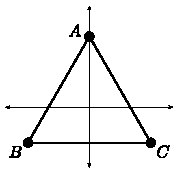
\includegraphics{../graphics/symTri.pdf}
\]
\begin{ques}
The matrix $\mat{R}_{360}$ will rotate this triangle completely
around the origin. What matrix will rotate this triangle one-third of
a complete rotation?
\end{ques}

As a gesture of friendship, I'll take this one. One-third of $360$ is
$120$. So we see that $\mat{R}_{120}$ will rotate the triangle one-third
of a full rotation. Do you remember this matrix? Here it is:
\[
\mat{R}_{120} =
\begin{bmatrix}
\frac{-1}{2} & \frac{-\sqrt{3}}{2} & 0\\
\frac{\sqrt{3}}{2} & \frac{-1}{2} & 0\\
0 & 0 & 1
\end{bmatrix}
\]
In spite of the fact that this matrix is messy and that matrix
multiplication is somewhat tedious, you should realize that
\[
\mat{R}_{120}^2 = \mat{R}_{240}\qquad\text{and}\qquad\mat{R}_{120}^3 = \mat{R}_{360}.
\]
Let's put these facts (and a few more) together in what is called a
\textit{group table}\index{group table}. Remember multiplication
tables from elementary school? Well, we're going to make something
like a ``multiplication table'' of rotations. We'll start by listing
the identity and powers of a one-third rotation along the top and
left-hand sides. Setting $\mat{R} = \mat{R}_{120}$ we have:
\[
{
\renewcommand{\arraystretch}{1.2}
\begin{array}{|c||c|c|c|c|c}
\hline 
\circ & \mat{I} & \mat{R} & \mat{R}^2 & \mat{R}^3 & \cdots \\ \hline\hline 
\mat{I} & & & & &  \\ \hline 
\mat{R} & & & & &  \\ \hline 
\mat{R}^2 &  & & & & \\ \hline
\mat{R}^3 &  & & & & \\ \hline
\vdots &  & & & & \\ 
\end{array}}
\]
Since $\mat{R}^3 = \mat{I}$, we need only take our table to
$\mat{R}^2$. At this point we can write out the complete table:
\[
{
\renewcommand{\arraystretch}{1.2}
\begin{array}{| c || c | c | c |}
\hline 
\circ & \mat{I} & \mat{R} & \mat{R}^2 \\ \hline\hline 
\mat{I} & \mat{I} & \mat{R} & \mat{R}^2 \\ \hline 
\mat{R} & \mat{R} & \mat{R}^2 & \mat{I} \\ \hline 
\mat{R}^2 & \mat{R}^2 & \mat{I} & \mat{R} \\ \hline
\end{array}}
\]
Since matrix multiplication is associative, and we see from the table
that every element has an inverse, we see that 
\[
\{\mat{I}, \mat{R}, \mat{R}^2\}
\]
is a group.

\begin{ques} 
What rotation matrices would we use when working with a square?  A
pentagon?  A hexagon?
\end{ques}
\QM


\subsection{Groups of Reflections}

Let's see another group. Again consider an equilateral triangle.  This
time we are interested in the three lines of reflection that preserve
this triangle:
\[
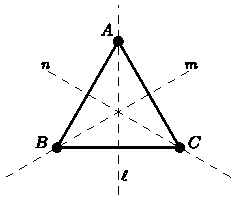
\includegraphics{../graphics/symTriRef.pdf}
\]

\begin{ques}
Suppose that the triangle above is centered at the origin of the
$(x,y)$-plane. What are equations for $\l$, $m$,
and $n$?
\end{ques}
\QM

The easiest of the reflections above is the reflection over
$\mat{F}_{\l}$.
\[
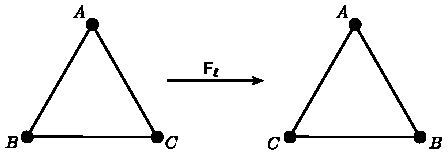
\includegraphics{../graphics/symTriRef1.pdf}
\]
We'll start our group table off with just two elements: $\mat{I}$ and
$\mat{F}=\mat{F}_{\l}$.

\[
\begin{array}{| c || c | c |}\hline
\circ & \mat{I} & \mat{F} \\ \hline\hline
\mat{I} & \mat{I} & \mat{F} \\\hline
\mat{F} & \mat{F} & \mat{I} \\ \hline
\end{array}
\]

Notice that when we apply $\mat{F}$ twice we're right back where we
started. Hence, $\mat{F} \mat{F} = \mat{I}$. Since matrix
multiplication is associative, we see that
\[
\{ \mat{I}, \mat{F} \}
\]
forms a group. Specifically this is a group of reflections of the
triangle.

\begin{ques} 
Above we used $\mat{F}_\l$. What would happen if we used $\mat{F}_m$
or $\mat{F}_n$? Also, what are the equations for the lines of symmetry
of the square centered at the origin?
\end{ques}
\QM







\subsection{Symmetry Groups}

Now let's mix our rotations and reflections.  Consider our original
triangle and apply $\mat{F}_\ell \mat{R}_{120}$:
\[
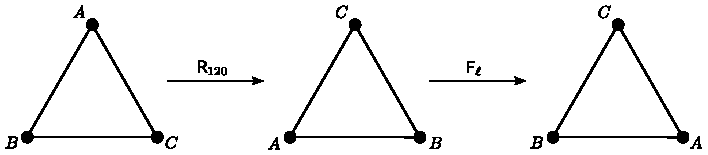
\includegraphics{../graphics/symTriComp1.pdf}
\]
What you may not immediately notice is that we obtain the same
transformation by taking the original triangle and applying
$\mat{F}_m$.
%\[
%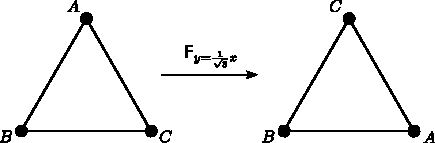
\includegraphics{../graphics/symTriComp2.pdf}
%\]



As it turns out, every possible symmetry of the equilateral triangle
can be represented using reflections and rotations.  Each of these
reflections and rotations can be expressed as a composition of a
single reflection and a single rotation.  The collection of all
symmetries forms a group called the \index{symmetry
  group}\textit{symmetry group} of the equilateral triangle. 
\[
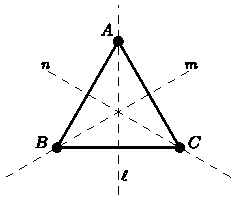
\includegraphics{../graphics/symTriRef.pdf}
\]
Let's see the group table, note we'll let $\mat{R} = \mat{R}_{120}$
and $\mat{F} = \mat{F}_{\l}$:

\[
{
\renewcommand{\arraystretch}{1.2}
\begin{array}{| c || c | c | c |c | c | c |}
\hline
\circ & \mat{I} & \mat{R} & \mat{R}^2  & \mat{F} & \mat{F} \mat{R} &  \mat{F} \mat{R}^2  \\ \hline \hline
\mat{I} & \mat{I} & \mat{R} & \mat{R}^2 & \mat{F} & \mat{F} \mat{R} & \mat{F} \mat{R}^2 \\ \hline
\mat{R} & \mat{R} & \mat{R}^2 & \mat{I} & \mat{F} \mat{R}^2 & \mat{F} & \mat{F} \mat{R} \\ \hline
\mat{R}^2 & \mat{R}^2 & \mat{I} & \mat{R} & \mat{F} \mat{R} & \mat{F} \mat{R}^2 & \mat{F}  \\ \hline
\mat{F} & \mat{F} & \mat{F} \mat{R} & \mat{F} \mat{R}^2 & \mat{I} & \mat{R} & \mat{R}^2 \\ \hline
\mat{F} \mat{R} & \mat{F} \mat{R} & \mat{F} \mat{R}^2 & \mat{F} & \mat{R}^2 & \mat{I} & \mat{R}  \\ \hline
\mat{F} \mat{R}^2 & \mat{F} \mat{R}^2 & \mat{F} & \mat{F} \mat{R} & \mat{R} & \mat{R}^2 & \mat{I}\\ \hline
\end{array}}
\]

This table shows every symmetry of the triangle, including the
identify $\mat{I}$. By comparing the rows and columns of the group
table, you can see that every element has an inverse. This combined
with the fact that the matrix multiplication is associative shows that
the symmetries of the triangle,
\[
\{ \mat{I},\mat{R},\mat{R}^2,\mat{F},\mat{F} \mat{R},  \mat{F} \mat{R}^2\}
\]
form a group.

\begin{ques} 
Can you express the symmetries of squares in terms of reflections
and rotations? What does the group table look like for the symmetry
group of the square?
\end{ques}
\QM



\newpage

\problems
\begin{enumerate}
\item State the definition of a group of matrices.
\item How many lines of reflectional symmetry exist for a square?
  Provide a drawing to justify your answer.
\item What are the equations for the lines of reflectional symmetry that exist for
  the square? Explain your answers.
\item How many lines of reflectional symmetry exist for a regular hexagon?  Provide a
  drawing to justify your answer.
\item What are the equations for the lines of reflectional symmetry
  for a regular hexagon?  Explain your answers.
%\item Give the group table for the rotations of a square.
%\item Give the group table for the rotations of a regular hexagon.
%\item Give the group table for the reflections of a square.
%\item Give the group table for the reflections of a regular hexagon.
%\item Give the group table for the symmetries of a square.
%\item Give the group table for the symmetries of a regular hexagon.
\item How many consecutive rotations are needed to return the vertexes
  of a square to their original position? Provide a drawing to justify
  your answer, labeling the vertexes.
\item How many degrees are in one-fourth of a complete rotation of the
  square?  Explain your answer.
\item How many degrees are in one-sixth of a complete rotation of the
  regular hexagon?  Explain your answer.
\item In this section, we've focused on a 3-sided figure, a 4-sided
  figure, and a 6-sided figure.  Why do we not include the rotation
  group for the pentagon in this section?  If we did, how many degrees
  would be in one-fifth of a complete rotation?
\item With notation used in this section, draw pictures representing
  the action of the following isometries $\mat{F}_\l$, $\mat{R}$,
  $\mat{R}\mat{F}_\l$ and $\mat{F}_\l\mat{R}$ on the equilateral
  triangle.
\item Consider a square centered at the origin. Draw pictures
  representing the action of $\mat{F}_{y=0}$, $\mat{R}_{90}$,
  $\mat{R}_{90}\mat{F}_{y=0}$, and $\mat{F}_{y=0} \mat{R}_{90}$ on
  this square.
\item Consider a hexagon centered at the origin. Draw pictures
  representing the action of $\mat{F}_{x=0}$, $\mat{R}_{60}$,
  $\mat{R}_{60}\mat{F}_{x=0}$, and $\mat{F}_{x=0} \mat{R}_{60}$ on
  this hexagon.
\item Find two symmetries of the equilateral triangle, neither of
  which is the identity, such that their composition is
  $\mat{R}_{120}$. Explain and illustrate your answer.
\item Find two symmetries of the equilateral triangle, neither of
  which is the identity, such that their composition is
  $\mat{F}_{x=0}$. Explain and illustrate your answer.
\item Find two symmetries of the equilateral triangle, neither of
  which is the identity, such that their composition is
  $\mat{R}_{120}^2$. Explain and illustrate your answer.
\item Find two symmetries of the square, neither of which is the
  identity, such that their composition is $\mat{R}_{180}$. Explain
  and illustrate your answer.
\item Find two symmetries of the square, neither of which is the
  identity, such that their composition is $\mat{F}_{\l}$. Explain
  and illustrate your answer.
\item Find two symmetries of the square, neither of which is the
  identity, such that their composition is $\mat{R}_{270}$. Explain
  and illustrate your answer.
\item Use a group table to help you write out the symmetries of the
  equilateral triangle. List all elements that commute with every
  other element in the table. Explain your reasoning.
\item Use a group table to help you write out the symmetries of the
  square. List all elements that commute with every other element in
  the table. Explain your reasoning.
\item Use a group table to help you write out the symmetries of the
  regular hexagon. List all elements that commute with every other
  element in the table. Explain your reasoning.
\item Let $\mat{M}$ be a symmetry of the equilateral triangle. Define
\[
C(\mat{M}) = \{\text{all symmetries that commute with $\mat{M}$}\}.
\]
Write out $C(\mat{M})$ for every symmetry $\mat{M}$ of the equilateral
triangle. Make some observations.
\end{enumerate}

